% End-semester B.Tech project report (IITD Applied Mechanics template, iitdamthes class)
%%%%%%%%%%%%%%%%%%%%%%%%%%%%%%%%%%%%%%%%%%%%%%%%%%%%%%%%%%%%%%%%%%%%%%%%%%%
\documentclass[12pt]{iitdamthes}
\usepackage[T1]{fontenc}
\usepackage{lmodern}
\usepackage{natbib}
\usepackage{graphicx}
\usepackage{amsmath}
\usepackage{booktabs}
\pagestyle{bfheadings}
\bibliographystyle{apalike}
\renewcommand{\bibname}{References}
\graphicspath{{figures/}}
\begin{document}

\begin{frontmatter}

\title{TURBULENT FLOW BEHIND A FLAT PLATE\\ MOUNTED NORMAL TO THE WALL}
\author{Ankit Kumar Modi \& Gaurav Waghmare}
\supervisor{Arjun Sharma}
\submitdate{November 2026}
\btech
\endsem
\tablespagetrue
\maketitle

\studentdeclaration
\supervisorcertificate

%%%%%%%%%%%%%%%%%%%%%%%%%%%%%%%%%%%%%%%%%%%%%%%%%%%%%%%%%%%%%%%%%%%%%%
\acknowledgements
We thank our supervisor, Prof.\ Arjun Sharma, for his guidance throughout the project, and in
particular for directing the second half of the work towards the physics of the wall--plate
junction. We also thank the Department of Applied Mechanics, IIT Delhi, for the computational
facilities and the ANSYS Fluent licence.

\noindent\textbf{Use of AI tools.} An AI assistant (Claude, Anthropic) was used during this work as a
step-by-step guide for setting up and checking the ANSYS Fluent simulations (meshing settings,
solver settings, monitors and post-processing procedures), to write the Python scripts used for
post-processing the exported data (boundary-layer integrals, grid-convergence index, vorticity
circulation and skin-friction statistics, and the plots in Figures 2 and 4--7), to suggest physical
interpretations of the results, and to draft and edit the text of this report. All simulations were
run by the authors; all numbers in this report come from our own simulation data, and the authors
checked the analysis and take full responsibility for the content.

% TODO (authors): update this paragraph to describe each author's contribution in the second half.
\prefacesection{Contribution of Authors}
The work was carried out jointly by both authors. [Authors: describe here who did the geometry and
meshing, the three-grid study, the Fluent post-processing and data export, and the writing.]

%%%%%%%%%%%%%%%%%%%%%%%%%%%%%%%%%%%%%%%%%%%%%%%%%%%%%%%%%%%%%%%%%%%%%%
\begin{abstract}
\sl
The turbulent flow in the corner formed by two flat plates joined at right angles (an L-shaped
wall--plate junction, 460~mm long, $Re_L = 1.1\times10^6$) is studied with steady RANS simulations
(ANSYS Fluent, SST $k$--$\omega$, $y^+<1$). Compared with the mid-semester study, the domain,
boundary conditions, mesh and solver were corrected, and a three-grid study
(0.53, 1.15 and 2.53 million cells, refinement ratio 1.30) gives a grid-convergence index of
4.6\% for the drag coefficient ($C_d = 0.0617$) and 2.7\% for the corner velocity. The analysis
focuses on the junction. The blunt leading edge produces a stagnation region that is strongest at
the inside corner and a separation bubble that reattaches 40--77~mm downstream. Because vortex
lines cannot end ($\nabla\cdot\boldsymbol{\omega}=0$), the wall vorticity of the floor and the
plate is tilted at the corner into streamwise vorticity, forming a symmetric pair of
counter-rotating corner vortices. They move fluid towards the corner along both walls and out
along the corner bisector, bring high-momentum fluid down onto each wall 15--30~mm from the
corner, and reduce the skin friction in the corner by 30--50\%. Their circulation decays nine-fold
between the leading and trailing edges. The limitation of the SST model for stress-induced
secondary flow is discussed.
\end{abstract}

\makecontents

%%%%%%%%%%%%%%%%%%%%%%%%%%%%%%%%%%%%%%%%%%%%%%%%%%%%%%%%%%%%%%%%%%%%%%
\notations
\begin{tabular}{@{}lp{0.68\textwidth}@{}}
$x, y, z$ & coordinates normal to the plate, normal to the floor, streamwise (flow in $-z$)\\
$u, v, w$ & mean velocity components in $x, y, z$\\
$U_\infty$ & inlet velocity, 36 m/s\\
$L$ & plate length, 460 mm\\
$\delta_{99}, \delta^*, \theta, H$ & boundary-layer, displacement, momentum thickness; $H=\delta^*/\theta$\\
$\boldsymbol{\omega}$, $\omega_x, \omega_y, \omega_z$ & vorticity vector and its components\\
$\Gamma^{\pm}$ & circulation of positive/negative streamwise vorticity in the corner\\
$C_f$, $C_d$ & skin-friction coefficient $\tau_w/\tfrac12\rho U_\infty^2$; drag coefficient\\
$y^+$ & wall distance in viscous units\\
$N$, $h$, $r$ & cell count, representative cell size $(V/N)^{1/3}$, refinement ratio\\
BOI & body of influence (local mesh refinement region)\\
GCI & grid convergence index \citep{celik2008}\\
LE, TE & leading edge, trailing edge\\
RANS, SST & Reynolds-averaged Navier--Stokes; shear-stress transport $k$--$\omega$ model\\
\end{tabular}

\end{frontmatter}

%%%%%%%%%%%%%%%%%%%%%%%%%%%%%%%%%%%%%%%%%%%%%%%%%%%%%%%%%%%%%%%%%%%%%%
\chapter{Introduction and Literature Review}
Wherever a body meets a wall --- a wing on a fuselage, a fin on a hull, a pier on a river bed ---
the boundary layers of the two surfaces meet in a corner. This \emph{junction flow} is
three-dimensional: vortices form at the leading edge, cross-stream (secondary) motion appears along
the corner, and the wall shear and drag there differ from those on either surface alone
\citep{simpson2001}. The project started from the experiment of \citet{nakayama1984}, who measured
the mean and secondary velocities, Reynolds stresses and skin friction behind a flat plate mounted
normal to a wall and found secondary motion that changes the wall shear near the junction.

Turbulent secondary flows are of two kinds \citep{bradshaw1987}. \emph{Prandtl's first kind} arises
when existing vorticity is tilted by the mean flow (pressure gradients, geometry) and can reach tens
of percent of the main velocity; the horseshoe vortex wrapped around the nose of a wing--body junction,
whose legs trail along the corners, is the classic example \citep{simpson2001}. The \emph{second kind}
is driven by the anisotropy of the Reynolds stresses in a straight corner \citep{gessner1973} and is
weak, about 1--3\% of the main velocity. The link between the two walls is kinematic: vorticity is
solenoidal, $\nabla\cdot\boldsymbol{\omega}=0$, so vortex lines cannot end in the fluid
\citep{saffman1992}; the spanwise vortex lines of one wall must turn into those of the other at the
corner and are partly tilted into the flow direction. The SST $k$--$\omega$ model \citep{menter1994}
is the standard RANS model for wall-bounded flows with separation, but as an isotropic eddy-viscosity
model it cannot produce the second kind \citep{pope2000}.

The mid-semester study was qualitative and unverified. The objectives of this phase were: (i) a
corrected and verified simulation of an L-shaped wall--plate junction, with a three-grid uncertainty
estimate \citep{celik2008}; (ii) an explanation, through the vorticity field and
$\nabla\cdot\boldsymbol{\omega}=0$, of how the floor and plate boundary layers meet and mix in the
corner; and (iii) a quantitative comparison of the corner with regions far from it.

%%%%%%%%%%%%%%%%%%%%%%%%%%%%%%%%%%%%%%%%%%%%%%%%%%%%%%%%%%%%%%%%%%%%%%
\chapter{Formulation and Methodology}

\section{Geometry, model and mesh}
The model (Figure~\ref{fig:geom}) is an L made of a vertical plate and a floor plate, each 460~mm
long, 320~mm wide and 10~mm thick with square edges, inside a box 200~cm long, 60~cm wide and
50~cm high (77~cm of free stream upstream and downstream). The inside corner runs along
$x=y=10$~mm, the leading edge (LE) is at $z=+0.23$~m, the flow is in $-z$, and
$Re_L=U_\infty L/\nu=1.13\times10^6$. The side faces are symmetry planes (open air; the mid-semester
duct walls had accelerated the flow to 41.8~m/s). The steady RANS equations are solved with SST $k$--$\omega$ in ANSYS Fluent
\citep{fluent2024}; Table~\ref{tab:setup} compares the settings with the mid-semester ones. The
tetrahedral mesh has 25 prism layers on every face of the L ($y^+<1$) and a body of influence (BOI)
refining the region around it. Three grids were made by scaling only the face size on the L and the
BOI size by about 1.45 (Table~\ref{tab:gci}).

\begin{figure}[t]
\centering
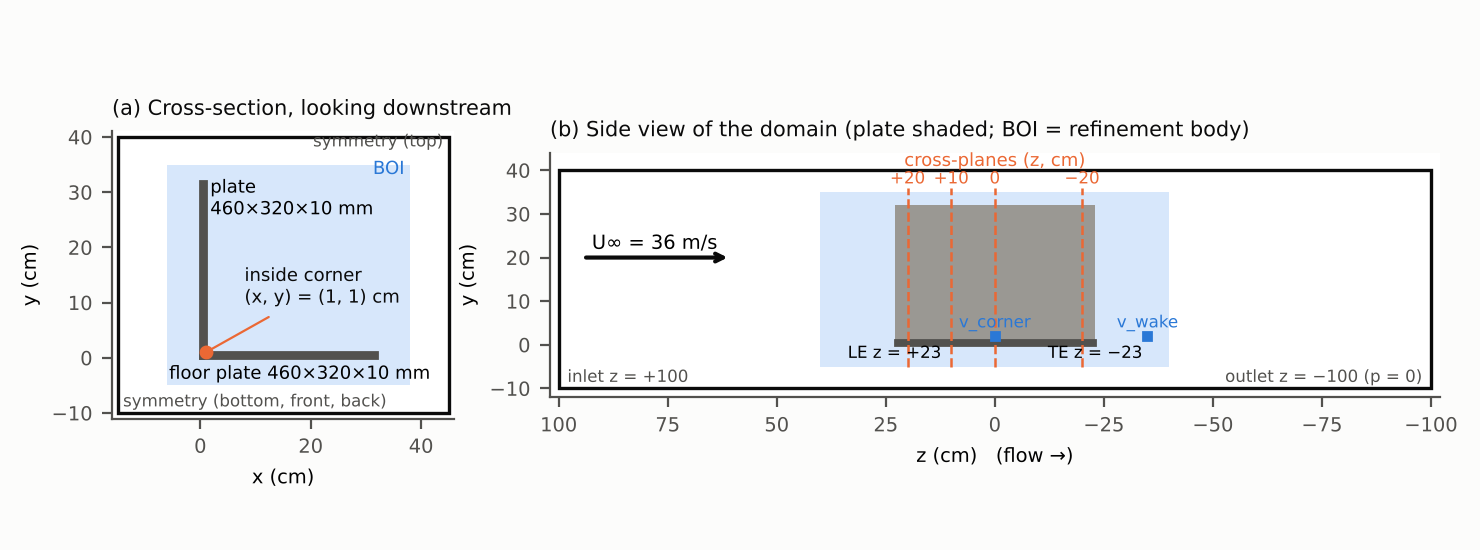
\includegraphics[width=0.9\textwidth]{geometry_domain.png}
\caption{Geometry, domain, refinement region (BOI), cross-planes and monitor points.}
\label{fig:geom}
\end{figure}

\begin{table}[t]
\centering
\small
\begin{tabular}{@{}p{0.17\textwidth}p{0.33\textwidth}p{0.43\textwidth}@{}}
\toprule
Item & Mid-semester & Final\\
\midrule
Model & T-shape in a small box & L-shaped junction (Fig.~\ref{fig:geom})\\
Side faces & no-slip walls (duct) & symmetry (open air)\\
Inlet / outlet & 36 m/s / 0 Pa & 36 m/s, 1\%, $\mu_t/\mu=10$ / 0 Pa\\
Outlet backflow & turbulence $10^{-14}$ & 5\%, $\mu_t/\mu=10$\\
Mesh & tetrahedral 10 mm, no inflation & 0.53--2.53 M cells, 25 layers from 0.01 mm\\
Solver & SIMPLE, relaxation 0.1/0.2 & coupled, pseudo-transient, 2nd order\\
Verification & none & convergence, mass balance, 3-grid GCI\\
\bottomrule
\end{tabular}
\caption{Settings before and after the mid-semester evaluation (air, $\rho=1.225$~kg/m$^3$,
$\mu=1.7894\times10^{-5}$~kg/(m\,s), SST $k$--$\omega$, no-slip L).}
\label{tab:setup}
\end{table}

\section{Analysis}
The corner flow is interpreted with the streamwise vorticity equation and the solenoidal condition,
\begin{equation}
\mathbf{u}\cdot\nabla\omega_z=\underbrace{\omega_x\frac{\partial w}{\partial x}
+\omega_y\frac{\partial w}{\partial y}}_{\text{tilting}}
+\underbrace{\omega_z\frac{\partial w}{\partial z}}_{\text{stretching}}+\text{diffusion},
\qquad \frac{\partial\omega_z}{\partial z}=-\left(\frac{\partial\omega_x}{\partial x}
+\frac{\partial\omega_y}{\partial y}\right).
\label{eq:vort}
\end{equation}
Profiles were taken at $z=0$ normal to each wall, 240~mm (far) and 10~mm (near) from the other
wall, and along the corner bisector. Data on four cross-planes ($z=+0.20, +0.10, 0, -0.20$~m, i.e.\
30--430~mm behind the LE) and on the walls were analysed in Python; the vortex strength is the
circulation $\Gamma^{\pm}=\int\omega_z\,dA$ of the positive and negative $\omega_z$ in a
$60\times60$~mm corner window (excluding 2~mm next to the walls).

%%%%%%%%%%%%%%%%%%%%%%%%%%%%%%%%%%%%%%%%%%%%%%%%%%%%%%%%%%%%%%%%%%%%%%
\chapter{Results and Discussion}

\section{Verification}
All grids converged: over the last 200 of 500 iterations $C_d$ varied by less than 0.05\% and the two
corner velocities by less than 0.9\%, the mass imbalance was below $2\times10^{-4}$\%, and the maximum
$y^+$ on the L was 0.77--0.93. $C_d$ and the corner velocity converge monotonically with the grid
(Table~\ref{tab:gci}); the change in $C_d$ from medium to fine is 1.4\% and the fine-grid GCI is
4.6\% for $C_d$ and 2.7\% for $v_{\rm corner}$. The corner-wake velocity is not monotonic and carries
about 6\% uncertainty --- it lies near the end of the BOI and is the most mesh-sensitive quantity.
All further results use the fine grid.

\begin{table}[t]
\centering
\small
\begin{tabular}{@{}lccccc@{}}
\toprule
Grid (face / BOI size) & $N$ (M) & $h$ (mm) & $C_d$ & $v_{\rm corner}$ (m/s) & $v_{\rm wake}$ (m/s)\\
\midrule
Coarse (10.6 / 25.5 mm) & 0.529 & 10.41 & 0.06373 & 33.20 & 28.57\\
Medium (7.3 / 17.5 mm) & 1.150 & 8.04 & 0.06253 & 29.55 & 27.16\\
Fine (5.0 / 12.0 mm) & 2.528 & 6.18 & 0.06165 & 28.30 & 25.60\\
\midrule
Apparent order $p$ & & & 1.25 & 4.2 & not monotonic\\
Extrapolated value & & & 0.0594 & 27.7 & ---\\
GCI$_{\rm fine}$ & & & \textbf{4.6\%} & \textbf{2.7\%} & ($\approx$6\% spread)\\
\bottomrule
\end{tabular}
\caption{Grid study ($r_{21}=r_{32}=1.30$; means over the last 200 iterations; monitor points in
Fig.~\ref{fig:geom}).}
\label{tab:gci}
\end{table}

\section{Leading edge of the junction}
The inlet total pressure is 819~Pa (794~Pa dynamic plus 25~Pa static). The highest pressure on the L
(837~Pa on nodes; a 2\% overshoot at the sharp stagnation edge) is on the blunt front face, and
iso-surfaces show that the stagnation region is largest at the \emph{inside corner} of the face,
where the oncoming fluid is blocked by both plates. The flow accelerates around the square edges (up
to $1.24U_\infty$) and separates. On the floor the wall shear is reversed up to 70--77~mm behind the
LE far from the plate but only 40--50~mm within 30~mm of it (Figure~\ref{fig:cf}a): the separation
bubble is shorter in the junction.

\section{Boundary layers far from and near the junction}
Far from the junction both boundary layers are alike at mid-length (Figure~\ref{fig:bl}):
$\delta_{99}=25.6$ and 26.0~mm, $\delta^*\approx6.2$~mm, $\theta\approx3.8$~mm, $H\approx1.65$. They are
far thicker than the flat-plate estimate $0.37xRe_x^{-1/5}\approx6$~mm \citep{schlichting2017} and $H$
exceeds the equilibrium value (1.3--1.4), because the layers are still recovering from the LE
separation; the edge velocity is 4\% above $U_\infty$ owing to displacement. Near the junction the
profiles are fuller close to the wall (28.4 against 26.0--26.7~m/s at 10~mm, +6--9\%) but never reach
the edge velocity, because they lie inside the other wall's boundary layer. Along the bisector, 99\%
of the edge velocity is reached 27~mm from the corner, whereas two superposed boundary layers would
need $\sqrt2\,\delta_{99}\approx36$~mm: the corner holds more momentum than superposition predicts,
which points to a secondary flow.

\begin{figure}[t]
\centering
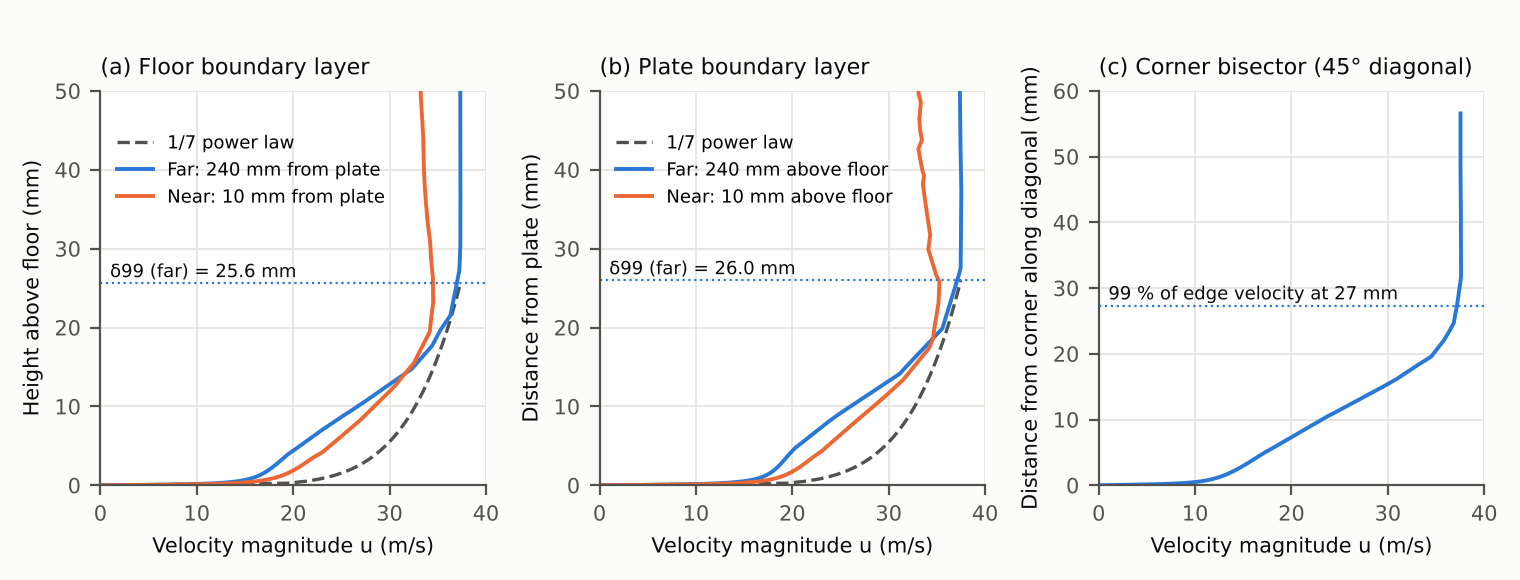
\includegraphics[width=0.92\textwidth]{stepA_profiles.png}
\caption{Velocity profiles at mid-length, far from (240~mm) and near (10~mm) the junction, and along
the corner bisector.}
\label{fig:bl}
\end{figure}

\section{Vorticity at the corner}
The floor boundary layer carries $\omega_x<0$ and the plate $\omega_y>0$, both about
$2\times10^5$~s$^{-1}$ at the wall ($\approx u_\tau^2/\nu$). At $z=0$ the $\omega_x$ layer thins near
the plate and the $\omega_y$ layer weakens towards the floor: the floor's vortex lines turn into the
plate's. There $\partial\omega_x/\partial x+\partial\omega_y/\partial y\neq0$, so by
equation~(\ref{eq:vort}) $\omega_z$ must vary along the corner, and the tilting terms are non-zero only
where both walls are close. Figure~\ref{fig:wz} shows the result. Inside the LE bubble ($z=+0.20$)
$\omega_z$ is strong and patchy; behind it a clean, nearly symmetric pair remains --- positive along
the plate, negative above the floor, centred 5--20~mm from the walls. Its circulation falls from
$\Gamma^{\pm}=+160/-145$ to $+53/-29$, $+29/-19$ and $+18/-14\times10^{-3}$~m$^2$/s: a nine-fold decay as
turbulent diffusion in the thickening boundary layers weakens the vortices. The vortices are therefore
generated near the LE, where stagnation and separation tilt the wall vorticity most strongly --- a
secondary flow of the first kind.

\begin{figure}[t]
\centering
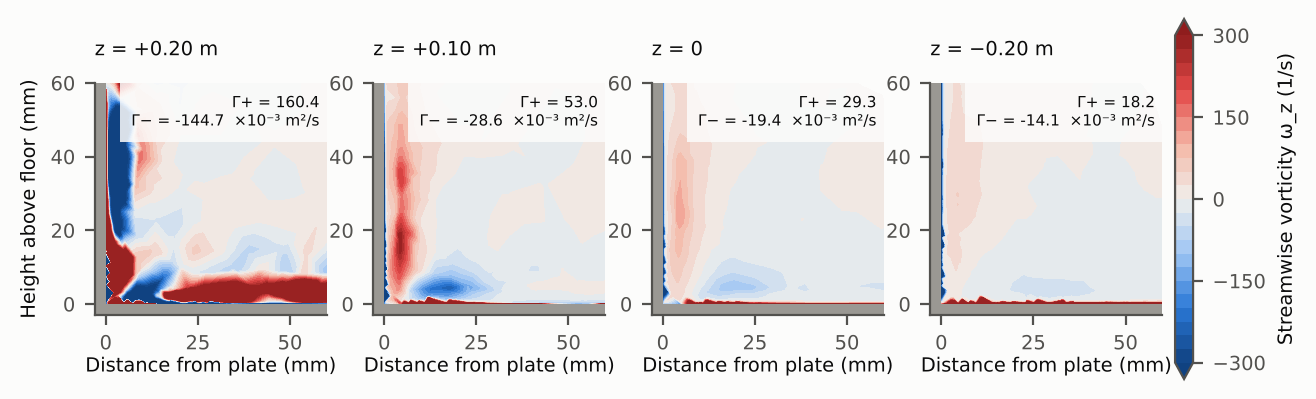
\includegraphics[width=\textwidth]{stepB_wz_planes.png}
\caption{Streamwise vorticity in the inside corner at $z=+0.20, +0.10, 0, -0.20$~m (30, 130, 230 and
430~mm behind the LE), with the circulation of its positive and negative parts ($\times10^{-3}$~m$^2$/s).}
\label{fig:wz}
\end{figure}

\section{Secondary flow and mixing in the corner}
Figure~\ref{fig:sec} shows what the pair does. At $z=+0.10$ and 0 the cross-flow within 3~mm of
each wall points \emph{towards} the corner (0.1--0.46~m/s) and along the bisector \emph{away} from it
(0.07--0.28~m/s). Each vortex sweeps slow fluid along its wall into the corner and lifts it out along
the bisector, and on its outer side brings fast fluid down onto the wall 15--30~mm from the corner;
the floor-side vortex turns in the same sense as a horseshoe-vortex leg \citep{simpson2001}. The
isovels are pushed towards the walls beside the corner, explaining the fuller profiles and the short
bisector distance above. At $z=+0.20$ the cross-flow is about ten times stronger (3.5~m/s) and points
away from the L (displacement by the blunt nose); at $z=-0.20$ it converges towards the walls ahead of
the trailing edge.

\begin{figure}[t]
\centering
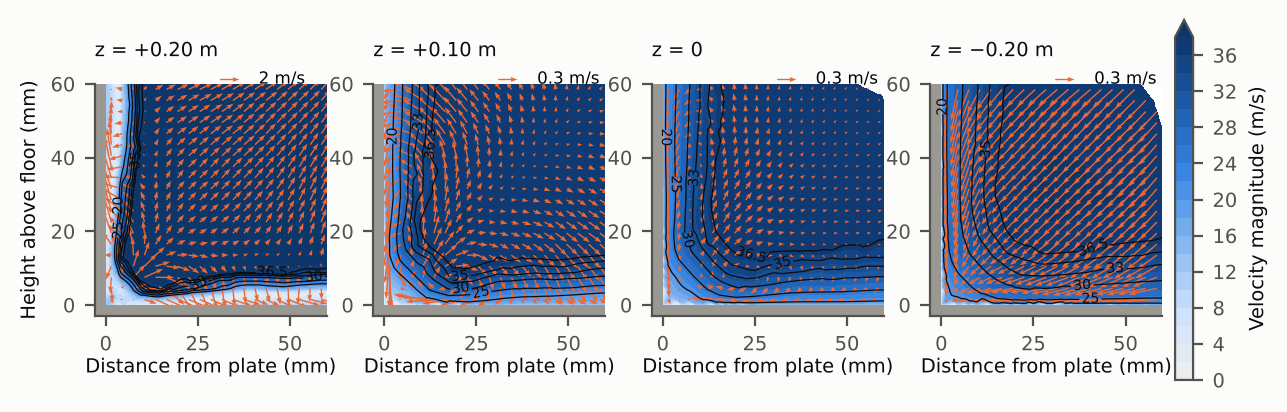
\includegraphics[width=\textwidth]{stepD_isovels_vectors.png}
\caption{Isovels (black, m/s) and cross-flow vectors in the inside corner at the same four stations
(reference arrow above each panel; the $z=+0.20$~m panel uses a scale about seven times larger).}
\label{fig:sec}
\end{figure}

\section{Wall shear stress}
The secondary flow leaves a clear imprint on the skin friction (Figure~\ref{fig:cf}). Within 4~mm of
the corner, where slow fluid collects, $C_f$ is 30--50\% lower than 60--150~mm away (e.g.\
$1.05\times10^{-3}$ against $2.16\times10^{-3}$ on the floor at $z=+0.10$). In the band 15--30~mm from
the corner, where fast fluid is brought down, $C_f$ is up to 32\% higher near the front, fading to
+8\% at $z=-0.20$ together with the vortices. Away from the corner $C_f$ rises along the plate as the
boundary layer recovers from the separation.

\begin{figure}[t]
\centering
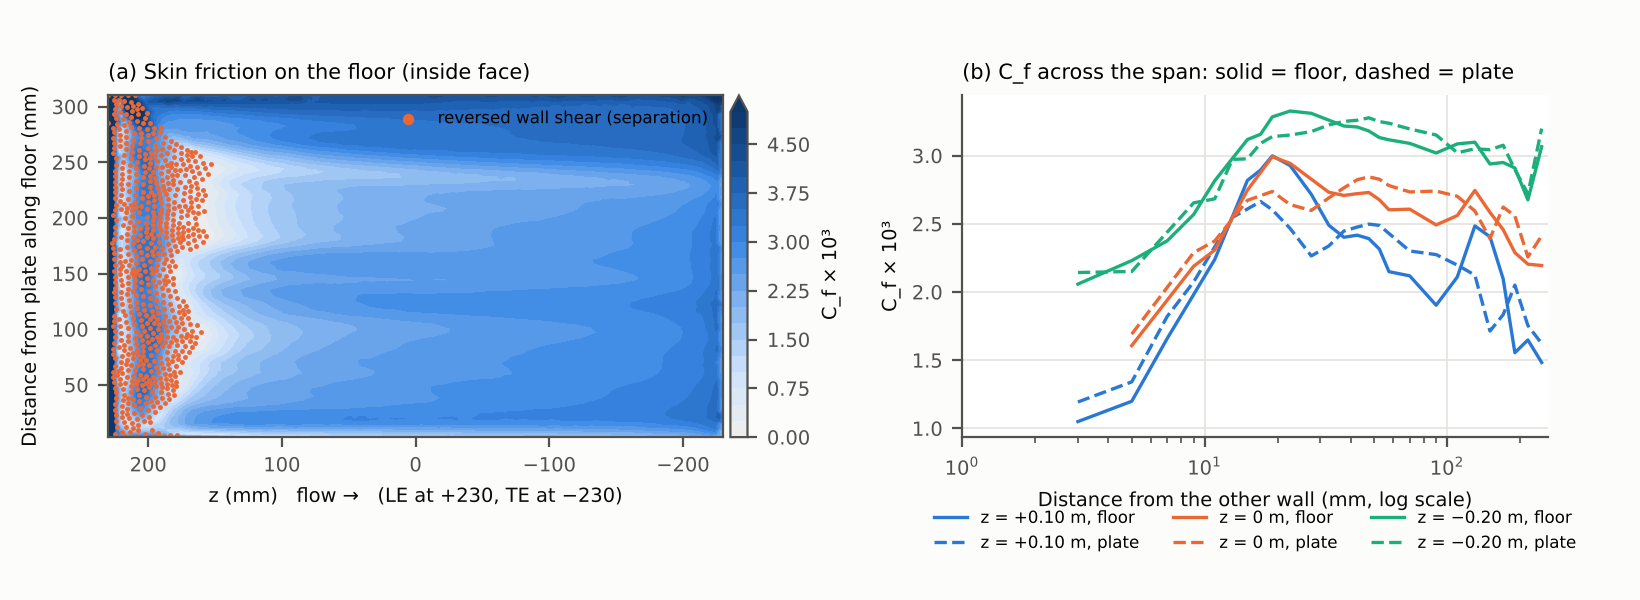
\includegraphics[width=0.92\textwidth]{stepE_cf.png}
\caption{(a) Skin friction on the inside face of the floor, with reversed wall shear marked;
(b) $C_f$ against distance from the other wall at three stations.}
\label{fig:cf}
\end{figure}

\noindent\textbf{Relation to the reference experiment.} In \citet{nakayama1984} a thick wall boundary
layer arrives from upstream and feeds a strong horseshoe vortex; here both boundary layers start at
the same blunt LE, so the corner vortices come from the LE stagnation and separation. The comparison is
therefore qualitative: both flows show streamwise corner vortices, momentum redistribution and a local
change of wall shear at the junction.

%%%%%%%%%%%%%%%%%%%%%%%%%%%%%%%%%%%%%%%%%%%%%%%%%%%%%%%%%%%%%%%%%%%%%%
\chapter{Conclusions and Future Work}
\begin{enumerate}
\item A verified RANS model of the L-junction ($y^+<1$, three grids, $r=1.3$) gives
$C_d=0.0617\pm4.6\%$ and a corner velocity converged to 2.7\%.
\item The blunt LE gives a stagnation region strongest at the inside corner and a separation bubble
shorter near the junction (40--50~mm) than far from it (70--77~mm).
\item Because $\nabla\cdot\boldsymbol{\omega}=0$, the floor and plate vortex lines join through the
corner and are tilted into a symmetric pair of counter-rotating streamwise vortices, whose
circulation decays nine-fold from the LE to the trailing edge.
\item The pair moves slow fluid along the walls into the corner and out along the bisector, and fast
fluid onto the walls 15--30~mm away: $C_f$ is 30--50\% lower in the corner and up to 32\% higher beside it.
\end{enumerate}
\noindent\textbf{Limitations and future work.} SST cannot produce stress-induced secondary flow
(second kind, 1--3\% of the main velocity). Near the LE our cross-flow is about 10\% of $U_\infty$ and
the first kind dominates; downstream it is about 1\%, so details there carry model uncertainty. Next: SST corner-flow correction or a Reynolds-stress model, a finer corner-wake mesh, an incoming
wall boundary layer to compare quantitatively with \citet{nakayama1984}, and the NACA~0010 wing--body
junction.

\bibliography{references}

\end{document}
